\documentclass{beamer} 

\usepackage{graphicx}
\usepackage{subfigure}

%\usepackage{xeCJK} % 中文包
\usetheme{Boadilla}  
\usecolortheme{seagull} 

%\setbeamertemplate{caption}[numbered] % 序号
%\setbeamercovered{transparent=15}
\setbeamersize{text margin left=0.6cm, text margin right=0.6cm} % 设置页边距
\setbeamercovered{transparent} 
\setbeamertemplate{navigation symbols}{} %Navigationsleiste ausschalten     


\title{Weekly work summary}
\author{Guangzhi Ren}
\institute {}
\date{\today}

\begin{document}
	
\begin{frame}
	\titlepage   
\end{frame}


\begin{frame}{content}
\begin{itemize}
%	\item revisiting to former simulation result
	\item simulation of electromagnetic 5-field landau fluid using spectral method
	\begin{itemize}
%		\item conservation test
%		\item initial perturbation
%		\item parallel computation scheme
		\item Fourier transform and relevant treatment in the simulation 
	\end{itemize}
\end{itemize}
\end{frame}
%


\begin{frame}{Spectral Method(Fourier transform )}
	\begin{equation}
		\begin{aligned}
			& forward: f(m) = \frac{1}{N}\sum_{n=0}^{N-1}f(n)e^{-i2\pi{m}n/N}	\\
			& backward: f(n) = \sum_{m=0}^{N-1}f(m)e^{i2\pi{m}n/N}
		\end{aligned}
	\end{equation}
	\begin{equation}
		\begin{aligned}
			& f(k) = \frac{1}{N}\sum_{n=0}^{N-1}f(x)e^{-i2\pi{m}x/L_x}
			\sim\frac{1}{N}\sum_{n=0}^{N-1}f(x)e^{-ik_xx}	\\
			& f(x) = \sum_{m=0}^{N-1}f(k)e^{i2\pi{m}x/L_x}
			\sim\sum_{m=0}^{N-1}f(k)e^{ik_xx}
		\end{aligned}
	\end{equation}
\end{frame}

\begin{frame}
	for linear terms $L(x)$:
	\begin{equation}
		\mathcal{F}(L(x))= L_k(k)
	\end{equation}
	
	for nonlinear terms $A(x)B(x)$:
	\begin{equation}
		\begin{aligned}
			\mathcal{F}(A(x)B(x))
			&=\mathcal{F}[\mathcal{F}^{-1}(A_k(k))\cdot\mathcal{F}^{-1}(B_k(k))]	\\
			&\sim A_k(k)\ast B_k(k)
		\end{aligned}
	\end{equation}
	if $1/N$ in forward process, $$\mathcal{F}(A(x)B(x))= A_k(k)\ast B_k(k)$$
	
	if $1/N$ in backward process, $$\mathcal{F}(A(x)B(x))= \frac{1}{N}A_k(k)\ast B_k(k)$$
\end{frame}


\begin{frame}{1D Fourier Transform using FFTW3}
	\begin{equation}
		\begin{aligned}
			f(x)=1+\sin(5x)+2\sin(10x), x\in[0,2\pi] \\
			i.e. f(n)=1+\sin(5\frac{2\pi{n}}{N})+2\sin(10\frac{2\pi{n}}{N}), n\in[0,N]
		\end{aligned}
	\end{equation}
	
	\begin{figure}[H]
		\centering
		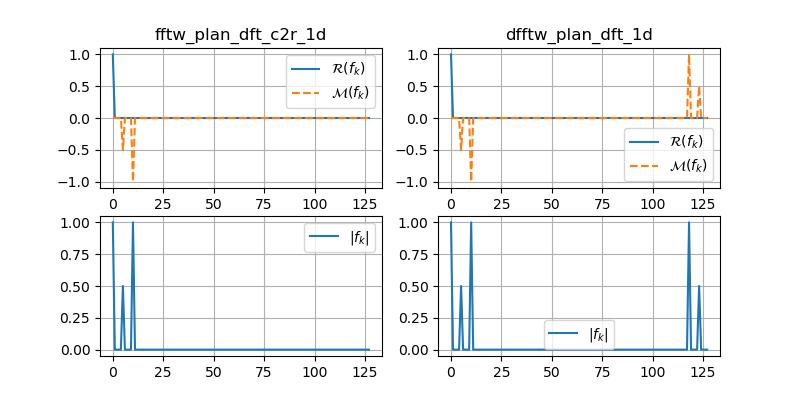
\includegraphics[width=0.8\textwidth]{./images/1d_k.png}
		\caption{}
	\end{figure}

\end{frame}

\begin{frame}{1D Fourier Transform using FFTW3}
	\begin{equation}
		\begin{aligned}
			m\in[0,1..N/2-1,-N/2,..-1] \\
			k_x\in[0,1\frac{2\pi}{L_x}...-1\frac{2\pi}{L_x}]
		\end{aligned}
	\end{equation}

	\begin{figure}[H]
		\centering
		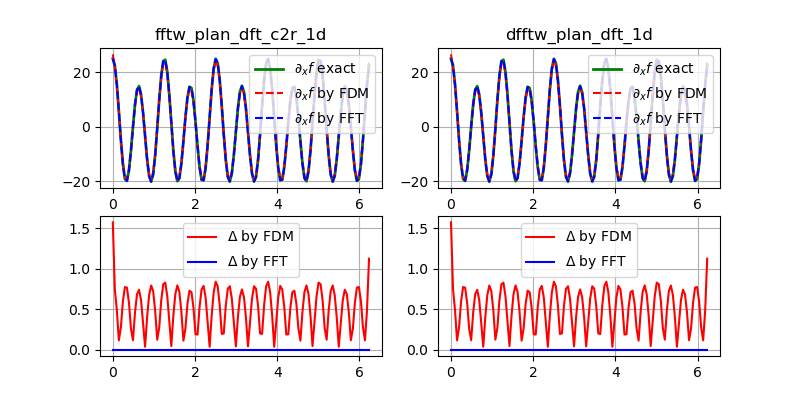
\includegraphics[width=0.8\textwidth]{./images/1d_d.png}
		\caption{}
	\end{figure}

\end{frame}


\begin{frame}{2D Parallel Fourier Transform using P3DFFT}
	2D FFT,
	\begin{equation}
		\begin{aligned}
			&f(m,n) = \frac{1}{MN}
			\sum_{y=0}^{M-1}[\sum_{z=0}^{N-1}
			f(\theta,\phi)e^{-i2\pi{n}z/N}]e^{-i2\pi{m}y/M}	\\
			&f(y,z) = \sum_{m=0}^{M-1}[\sum_{n=0}^{N-1}
			f(m,n)e^{i2\pi{n}z/N}]e^{i2\pi{m}y/M}
			=\sum_{m=0}^{M-1}\sum_{n=0}^{N-1}f(m,n)e^{i{m\theta+n\zeta}}
		\end{aligned}
	\end{equation}

	in P3DFFT output,	
	\begin{equation}
		\begin{aligned}
			m\in[0,1..M/2-1,-M/2,..-1] \\
			n\in[0,1,2,..N/2-1]
		\end{aligned}
	\end{equation}
	
\end{frame}


\begin{frame}{2D Parallel Fourier Transform using P3DFFT}
	\begin{figure}[H]
		\centering
		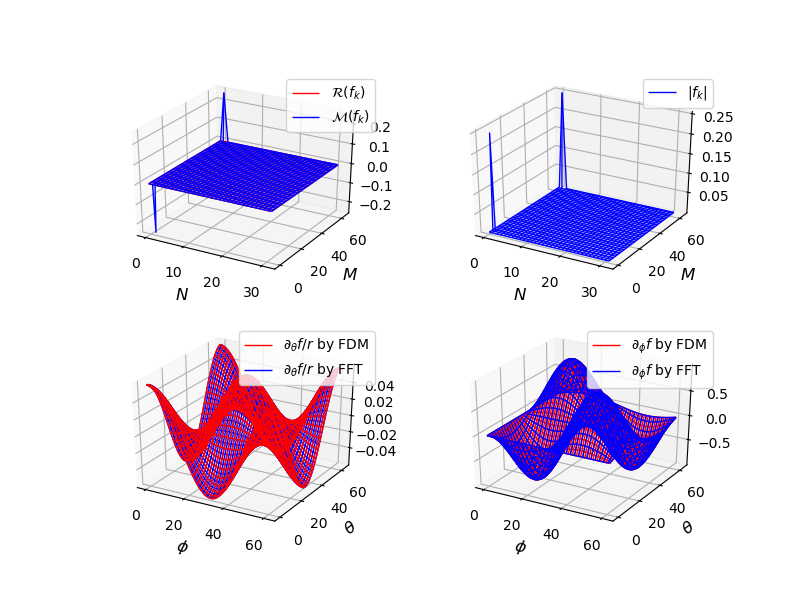
\includegraphics[width=0.8\textwidth]{./images/2d_kd.png}
		\caption{}
	\end{figure}
\end{frame}


\begin{frame}{Result Comparision of poisson bracket calculation}
	
	\begin{figure}[H]
		\centering
		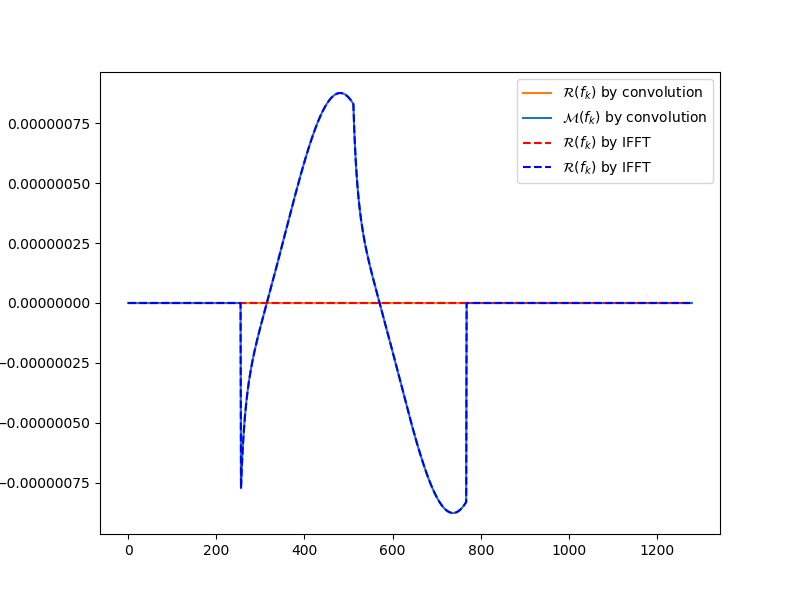
\includegraphics[width=0.8\textwidth]{./images/poisson.png}
		\caption{$[n,\phi]$ in different method for poisson bracket calculation}
	\end{figure}
	
\end{frame}


\begin{frame}
		\begin{figure}[H]
		\centering
		\subfigure[$\beta=0.1\%$]{
			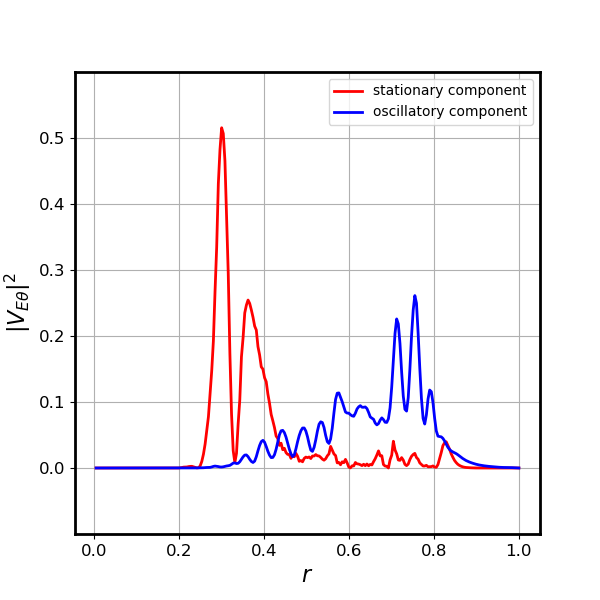
\includegraphics[width=0.2\textwidth]{./images/zf_filter_b01.png} 
		}
		\subfigure[$\beta=0.3\%$]{
			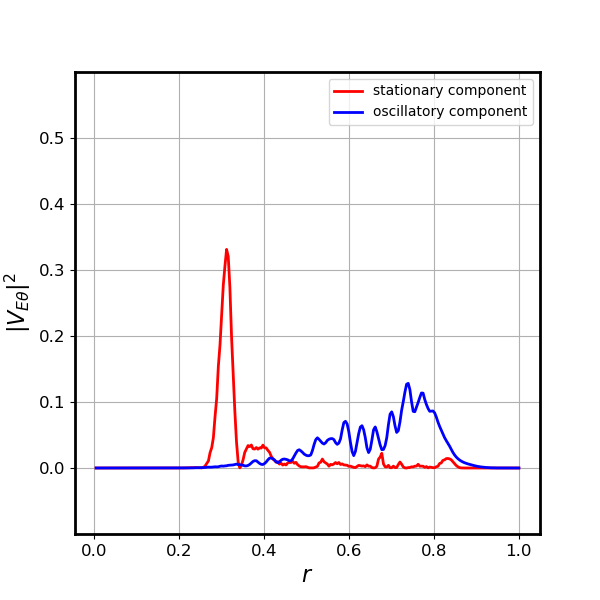
\includegraphics[width=0.2\textwidth]{./images/zf_filter_b03.png}
		}
		\subfigure[$\beta=1.0\%$]{
			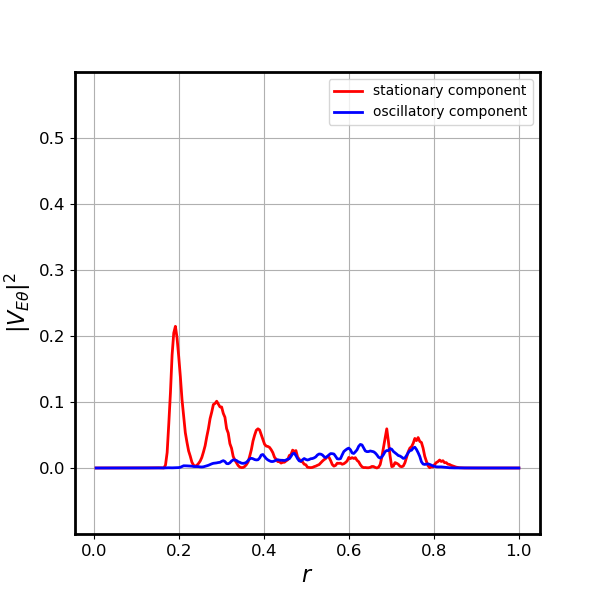
\includegraphics[width=0.2\textwidth]{./images/zf_filter_b10.png}
		}
		\subfigure[$\beta=1.2\%$]{
			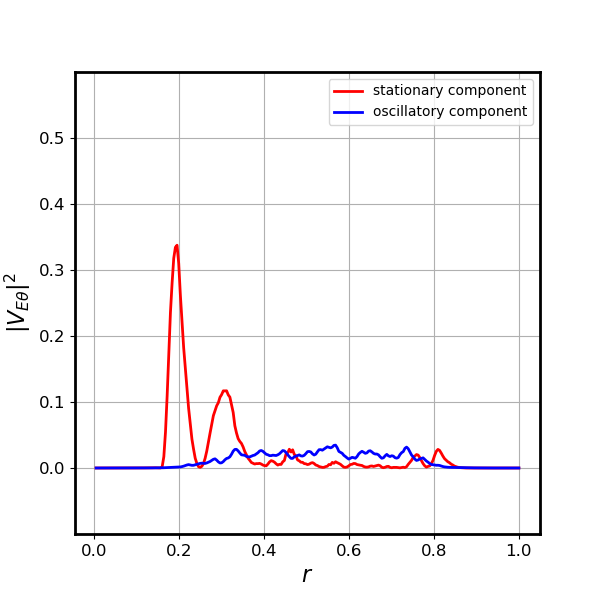
\includegraphics[width=0.2\textwidth]{./images/zf_filter_b12.png}
		}
		\caption{ Time averaged zonal flow profile }
	\end{figure}

	\begin{figure}[H]
		\centering
		\subfigure[$\beta=0.1\%$]{
			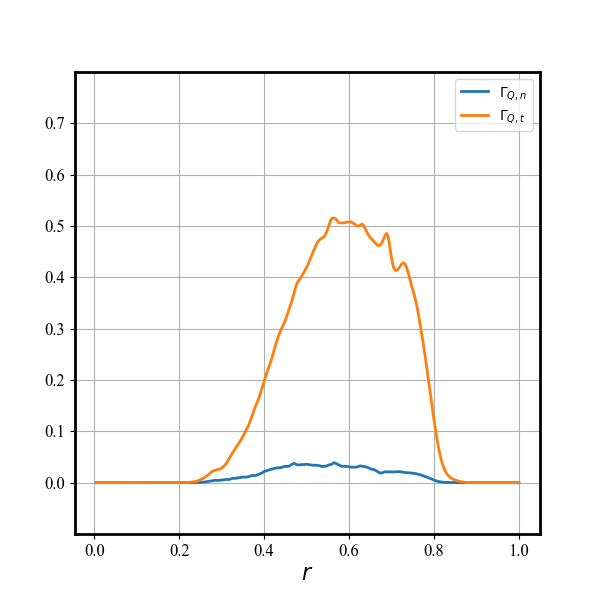
\includegraphics[width=0.2\textwidth]{./images/flux_b01.png} 
		}
		\subfigure[$\beta=0.3\%$]{
			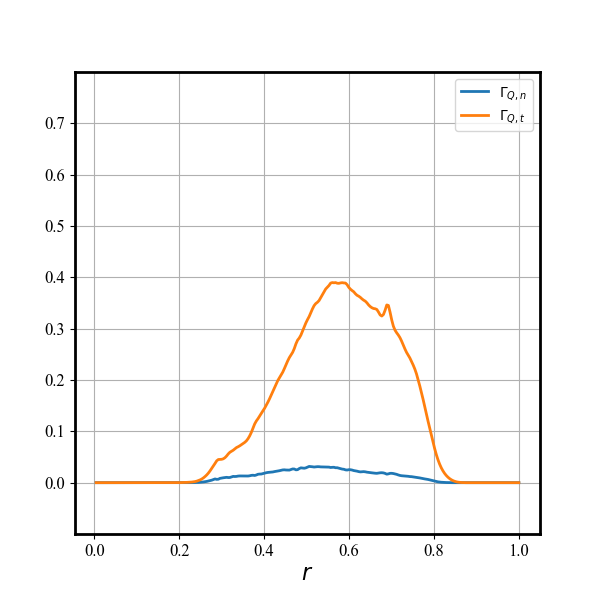
\includegraphics[width=0.2\textwidth]{./images/flux_b03.png}
		}
		\subfigure[$\beta=1.0\%$]{
			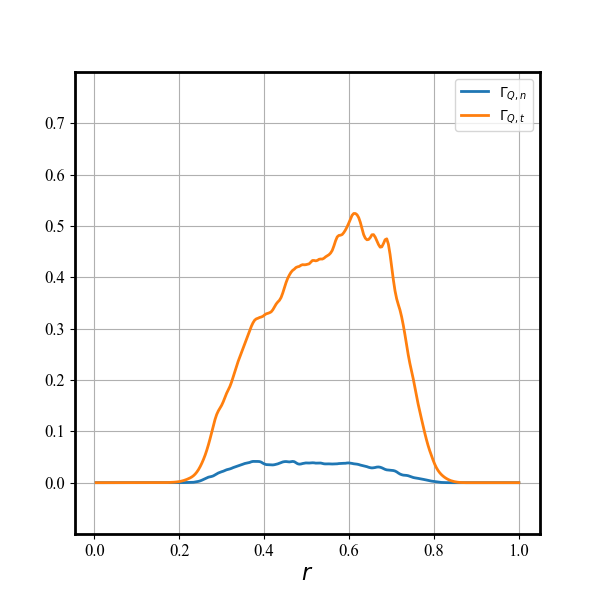
\includegraphics[width=0.2\textwidth]{./images/flux_b10.png}
		}
		\subfigure[$\beta=1.2\%$]{
			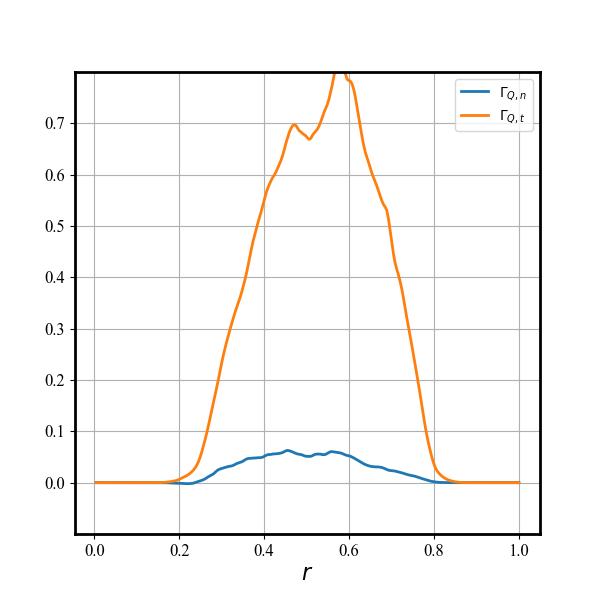
\includegraphics[width=0.2\textwidth]{./images/flux_b12.png}
		}
		\caption{ Time averaged transport flux profile }
	\end{figure}

\end{frame}


\begin{frame}{}
\begin{figure}[H]
	\centering
	\subfigure{
		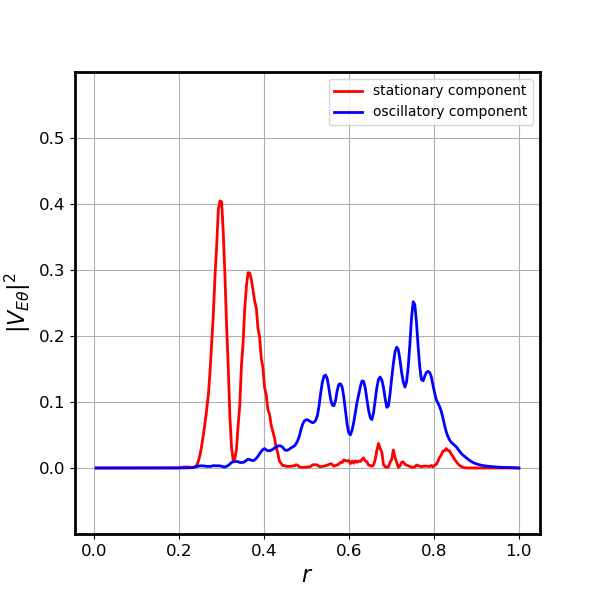
\includegraphics[width=0.25\textwidth]{./images/zf_filter_b01_m.png} 
	}
	\subfigure{
		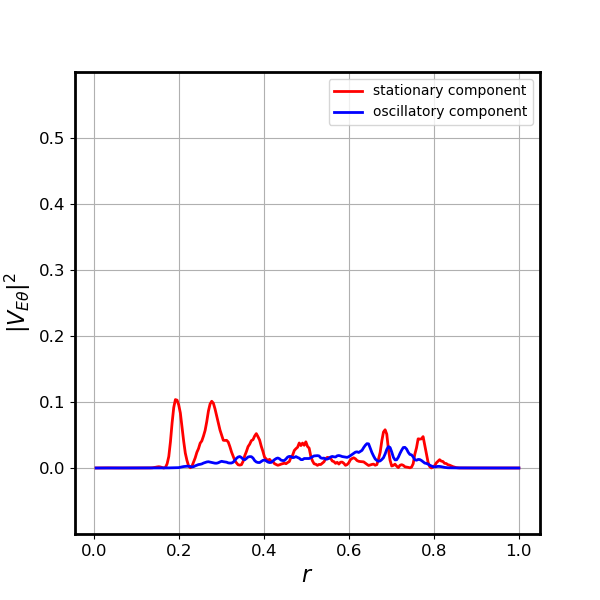
\includegraphics[width=0.25\textwidth]{./images/zf_filter_b10_m.png}
	}

	\subfigure{
		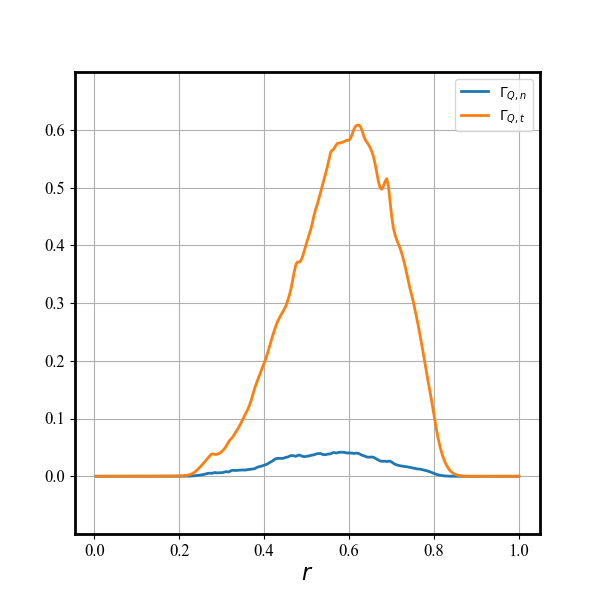
\includegraphics[width=0.25\textwidth]{./images/flux_b01_m.png} 
	}
	\subfigure{
		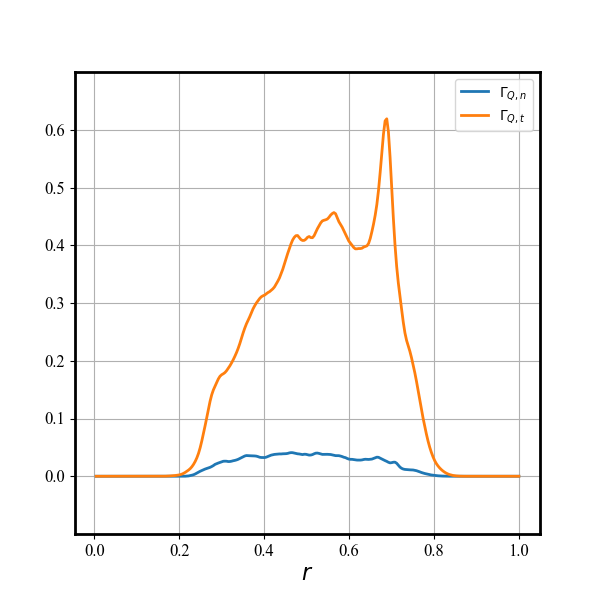
\includegraphics[width=0.25\textwidth]{./images/flux_b10_m.png}
	}
	\caption{  }
\end{figure}
\end{frame}



\end{document}